\documentclass[11pt, oneside]{article}   	

%%%%%%%%%%%%%%%%%%%%%%%%%%%%%%%%%%
% Packages
%%%%%%%%%%%%%%%%%%%%%%%%%%%%%%%%%%
\usepackage[colorlinks,citecolor=blue,urlcolor=blue,filecolor=blue,backref=page]{hyperref}

\usepackage{geometry}                	
\geometry{a4paper}                   	

\usepackage{graphicx}	
\usepackage{float}
\usepackage{subfig}

\usepackage{amsthm}
\usepackage{amsmath}							
\usepackage{amssymb}
\usepackage[utf8]{inputenc}

\usepackage{natbib}

\usepackage{url}

\usepackage{commath}

%%%%%%%%%%%%%%%%%%%%%%%%%%%%%%%%%%
% Macros
%%%%%%%%%%%%%%%%%%%%%%%%%%%%%%%%%%

\newcommand{\thetab}{{\boldsymbol{\theta}}}
\newcommand{\thetaHat}{{\hat{\thetab}}}
\newcommand{\alphab}{{\boldsymbol{\alpha}}}
\newcommand{\betab}{{\boldsymbol{\beta}}}
\newcommand{\mub}{\boldsymbol{\mu}}
\newcommand{\Sigmab}{\boldsymbol{\Sigma}}
\newcommand{\xib}{{\boldsymbol{\xi}}}
\newcommand{\xitildeb}{{\boldsymbol{\tilde{\xi}}}}
\newcommand{\pnorm}{p}
\newcommand{\pnn}{\phi}
\newcommand{\pnnj}{f}
\newcommand{\pdata}{p_{ \mathbf x}}
\newcommand{\pnoise}{p_{ \mathbf y}}
\newcommand{\pcondnoise}{p_{\y|\x}}
\newcommand{\palpha}{p_\alphab}
\newcommand{\pbeta}{p_\betab}

\newcommand{\Ib}{\boldsymbol{I}}
\renewcommand{\u}{{\mathbf u}}
\newcommand{\x}{{\mathbf x}}
\newcommand{\y}{{\mathbf y}}
\newcommand{\z}{{\mathbf z}}
\newcommand{\w}{{\mathbf w}}
\newcommand{\ytilde}{\mathbf{\tilde{y}}}
\newcommand{\X}{{\mathbf X}}
\newcommand{\psib}{\boldsymbol{\psi}}

\renewcommand{\P}{\mathbb{P}}
\newcommand{\E}{\mathbb{E}}
\newcommand{\Ex}{\E_{\x}}
\newcommand{\Ey}{\E_{\y}}
\newcommand{\Ealpha}{\mathbb{E}_{\alphab}}
\newcommand{\Ebeta}{\mathbb{E}_{\betab}}

\newcommand{\J}{\mathcal{J}}


%%%%%%%%%%%%%%%%%%%%%%%%%%%%%%%%%%
% Latex settings
%%%%%%%%%%%%%%%%%%%%%%%%%%%%%%%%%%

\graphicspath{{./figs/}}


%%%%%%%%%%%%%%%%%%%%%%%%%%%%%%%%%%
% Text
%%%%%%%%%%%%%%%%%%%%%%%%%%%%%%%%%%

\title{Noise Contrastive Estimation with Unobserved Variables}
\author{Michael Gutmann}
\date{\today}						

\begin{document}
\maketitle

\section{Background}
\subsection{Estimation of unnormalised models}
The project is generally about estimating the parameters $\thetab$ of
an unnormalised model $\pnn(\u ; \thetab)$ from observed data $\X =
(\x_1,\ldots,\x_n)$. The observed data are assumed be independent
realisations of a $d$-dimensional random variable $\x \sim \pdata$.\footnote{$\x \sim \pdata$ means that the
random variable $\x$ follows (has) the probability density function $\pdata$.} A
model is unnormalised if its integral does not equal one for all
parameter values, that is if
 \begin{align}
   \int_{\u }\pnn(\u;\thetab) \dif \u &= Z(\thetab) \neq 1.
\label{eq:Zdef}
  \end{align}
The term $Z(\thetab)$ is called the partition function. By definition,
the partition function can be used to convert the
unnormalised model $\pnn(\u;\thetab)$ into a normalised model
$\pnorm(\u;\thetab)$,
\begin{align}
  \pnorm(\u;\thetab)&=\frac{\pnn(\u;\thetab)}{Z(\thetab)}, & \int_{\u }\pnorm(\u;\thetab) \dif\u & = 1.
\end{align}
The partition function, however, defined via the integral in \eqref{eq:Zdef}, and computing the integral analytically is
generally impossible and computing it numerically is most often
extremely expensive (``curse of dimensionality''). This is an issue because the partition function
plays an important role in maximum likelihood estimation.

Maximum likelihood estimation is a standard method to estimate
parametric models. It consists in maximising the log-likelihood
function $\ell(\thetab)$ with respect to $\thetab$. The log-likelihood
is
\begin{align}
\ell(\thetab) &= \sum_{i=1}^n \log \pnorm(\x_i;\thetab) = \sum_{i=1}^n \log \pnn(\x_i;\thetab) - n \log ( Z(\thetab) ),
\end{align}
so that $\ell(\thetab)$ cannot be computed if $Z(\thetab)$ cannot be
computed. This means that standard maximum likelihood estimation
cannot be used for estimation of unnormalised models. As unnormalised
models occur widely -- Markov random fields are typical examples --
alternative estimation methods are needed for unnormalised models
\citep[see ][for further discussion]{Gutmann2013b}.

\subsection{Noise-contrastive estimation}
Noise contrastive estimation (NCE) is a method to estimate
unnormalised models. NCE formulates the density estimation
problem as a classification problem where we learn to distinguish
between the observed data and some reference data (called the
``noise''). The noise are generated by the user from a known noise
distribution. The basic idea is that by solving the classification
problem, we learn the differences between the data and the noise, and
that we can then deduce the properties of the data from the learned
differences since the properties of the noise are known

In more detail, let $\y_i, i=1 \ldots m$, be the noise that were
independently drawn from $\pnoise$. The classification task is to
distinguish between the $\x_i$ and the $\y_i$. More precisely, the
task is to decide whether a test point $\u$ has been sampled from
$\pdata$ (class 1) or from $\pnoise$ (class 2). Logistic regression
solves this task by parametrising the probability for $\u$ to be from
$\pdata$ as
\begin{align}
  \P( \u \sim \pdata; \thetab ) &= \frac{1}{1+\nu \exp(-h(\u;\thetab))}, 
\end{align}
with $\nu = m/n$ and $h(\u;\thetab)$ being some function
para\-metrised by $\thetab$. The factor $\nu$ biases the decision
according to the relative frequencies of the $\x_i$ and $\y_i$. The
parameters of the regression function can be learned by maximising $J_n(\thetab)$,
\begin{align}
  J_n(\thetab)&= \frac{1}{n} \left\{\sum_{i=1}^{n} \log  \P( \x_i \sim \pdata; \thetab ) + \sum_{i=1}^{m} \log\left[1- \P( \y_i \sim \pdata; \thetab )\right]\right\}\\
  & = -\frac{1}{n} \left\{\sum_{i=1}^{n} \log \left[1+\nu \exp(-h(\x_i;\thetab))\right] + \sum_{i=1}^{m} \log \left[1+1/\nu \exp(h(\y_i;\thetab))\right]\right\},
  \label{eq:Jn}
\end{align}
which is the sample version of $J(\thetab)$,
\begin{equation}
  J(\thetab) = - \Ex  \log \left[1+\nu \exp(-h(\x;\thetab))\right] - \nu \Ey \log \left[1+1/\nu \exp(h(\y;\thetab))\right].
  \label{eq:J}
\end{equation}
The symbols $\Ex$ and $\Ey$ denote expectation with respect to $\pdata$ and $\pnoise$, respectively.

Noise-contrastive estimation makes use of the fact that $J(\thetab)$ is
maximised by the parameter value $\thetab$ for which
\begin{equation}
  h(\u;\thetaHat) = \log \frac{\pdata(\u)}{\pnoise(\u)},
\end{equation}
see \citep{Gutmann2012a}.\footnote{For a more direct proof, see the appendix of \url{https://michaelgutmann.github.io/assets/slides/Gutmann-2016-11-11.pdf}.}
There are no constraints in the optimisation problem. Hence, if $\pnoise$ is known in closed from and
$h(\u;\thetab)$ is specified as
\begin{equation}
  h(\u;\thetab) = \log \frac{\pnn(\u;\thetab)}{\pnoise(\u)},
  \label{eq:Gdef}
\end{equation}
the unnormalised model can be estimated by optimising $J$, or, in
practice $J_n$. The key point is that no assumption about
normalisation of the model is needed: We can work with an unnormalised
model and maximising $J$ will automatically scale it
correctly~\citep{Gutmann2012a}. This assumes that the unnormalised
model $\pnn(.|\thetab)$ is parametric such that its scale can vary
freely, which can always be achieved by introducing an additional
scaling parameter $c$
\begin{align}
  \thetab &\rightarrow (\thetab;c)&   \pnn(\u;\thetab) &\rightarrow \exp(c)\pnn(\u;\thetab).
\end{align}

NCE is being used in various applications: for example for models of
text \citep{Mnih2012}, images \citep{Gutmann2013}, for machine
translation \citep{Zoph2016}, or for product recommendation
\citep{Tschiatschek2016}.\footnote{These papers are \emph{not}
  required reading. They are not needed in any way for the project.} One difficulty
of NCE, however, is that the noise distribution $\pnoise$ needs to be
specified by the user. While the theory of NCE imposes only weak
conditions \citep[Section 2.4]{Gutmann2012a}, practical constraints
are that (1) we can draw samples from $\pnoise$ and that (2) we have
an analytical expression for $\pnoise$. We next consider an estimation
method that is inspired by NCE for which the noise distribution can be
constructed in an automated manner.


\section{Noise-contrastive estimation with unobserved variables}
We now assume that we do not have data on all variables of the model
$\pnorm(\u;\thetab)$. Equivalently, we assume that the unnormalised
model is defined as an intractable integral over the unobserved variables $\z$
\begin{align}
  \pnn(\u;\thetab) = \int \pnn(\u, \z;\thetab) \dif \z. \label{eq:unnorm-marginalisation}
\end{align}
We thus have
\begin{align}
  \pnorm(\u,\z;\thetab) &= \frac{\pnn(\u, \z;\thetab)}{Z(\thetab)}\\
  \pnorm(\u; \thetab) &= \int \pnorm(\u, \z;\thetab) \dif \z\\
&=  \frac{\int \pnn(\u, \z;\thetab) \dif \z}{Z(\thetab)}
\end{align}
where $Z(\thetab)$ is the partition function as in \eqref{eq:Zdef}.

As the marginalisation in \eqref{eq:unnorm-marginalisation} is assumed
intractable, $\pnn(\u;\thetab)$ is not available and noise-contrastive
estimation cannot be used as before. We next derive a lower bound on
$J(\thetab)$ that can be estimated as a sample average, and which we maximise instead of $J(\thetab)$.

\subsection{Lower bound for the first term in the NCE objective function}
We first re-write $ - \log [1+\nu \exp(-h(\u;\thetab))]$ by inserting the definition of $h$
\begin{align}
  - \log [1+\nu \exp(-h(\u;\thetab))] & =  - \log \left[1+\nu \exp \left(- \log \frac{\pnn(\u;\thetab)}{\pnoise(\u)}\right) \right]\\
  & =  - \log \left[1+\nu \exp \left( \log \frac{\pnoise(\u)}{\pnn(\u;\thetab)}\right) \right]\\
  & =  - \log \left[1+\nu  \frac{\pnoise(\u)}{\pnn(\u;\thetab)} \right] 
\end{align}
Let further
\begin{equation}
  r(\u;\thetab) = \exp(h(\u; \thetab)) = \frac{\pnn(\u;\thetab)}{\pnoise(\u)}
  \label{eq:r-def}
\end{equation}
and
\begin{equation}
  g(r) = -\log \left(1+\nu \frac{1}{r} \right),
\end{equation}
we then obtain
\begin{equation}
  - \log [1+\nu \exp(-h(\u;\thetab))]  = g(r(\u; \thetab)).
\end{equation}
The first derivative of $g$ with respect to $r$ is
\begin{align}
\dod{g}{r} &= \frac{-1}{1+\nu \frac{1}{r}}\frac{-\nu}{r^2}\\
&= \frac{\nu}{r^2+\nu r}
\end{align}
The second derivative of $g$ with respect to $r$ is thus
\begin{align}
\dod[2]{g}{r} &= -\nu \frac{2r +\nu}{(r^2+\nu r)^2},
\end{align}
which is always negative for $r>0$. The function $g(r)$ is thus concave.

We now introduce an auxiliary distribution $q_u(\z)$ over $\z$ and write
\begin{align}
  \pnn(\u; \thetab) &= \int \pnn(\u, \z;\thetab) \dif \z\\
  & = \int q_u(\z) \frac{\pnn(\u,\z; \thetab)}{q_u(\z)} \dif \z\\
  & = \E_{\z \sim q_u} \left[\frac{\pnn(\u,\z; \thetab)}{q_u(\z)}\right]
  \label{eq:phi-importance-sampling}
\end{align}
This corresponds to estimating $\pnn(\u,\thetab)$ by importance sampling. The subscript for $q_u(\z)$ is meant to indicate that we can use different auxiliary distributions for different values of $\u$.

We can thus write $r(\u; \thetab)$ as
\begin{align}
  r(\u;\thetab) &= \frac{1}{\pnoise(\u)}  \E_{\z \sim q_u} \left[\frac{\pnn(\u,\z; \thetab)}{q_u(\z)}\right] \\
  & =  \E_{\z \sim q_u} \left[\frac{\pnn(\u,\z; \thetab)} {q_u(\z)\pnoise(\u)} \right]
  \label{eq:r-importance-sampling}
\end{align}
and since $g$ is concave, we have
\begin{align}
  - \log [1+\nu \exp(-h(\u;\thetab))]  &= g(r(\u; \thetab)) \\
  & = g\left(\E_{\z \sim q_u} \left[\frac{\pnn(\u,\z; \thetab)} {q_u(\z)\pnoise(\u)} \right]\right)\\
  & \ge \E_{\z \sim q_u} g\left( \frac{\pnn(\u,\z; \thetab)} {q_u(\z)\pnoise(\u)} \right).
\end{align}
With the definition of $g$, we thus obtain
\begin{equation}
  - \log [1+\nu \exp(-h(\u;\thetab))]  \ge -\E_{\z \sim q_u} \log \left[1+\nu \frac{q_u(\z)\pnoise(\u)}{\pnn(\u,\z; \thetab)}\right].
\end{equation}
We now plug this relation into $J(\thetab)$ in \eqref{eq:J}, where the values $\u$ are given by the values of the random vector $\x$. We thus write $q(\z|\x)$ instead of $q_u(\z)$. Doing so, we obtain 
\begin{align}
  J(\thetab)  &= - \Ex  \log \left[1+\nu \exp(-h(\x;\thetab))\right] - \nu \Ey \log \left[1+1/\nu \exp(h(\y;\thetab))\right]\\
  & \ge  -\Ex \E_{\z \sim q(\z|\x)} \log \left[1+\nu \frac{q(\z|\x)\pnoise(\x)}{\pnn(\x,\z; \thetab)}\right] -  \nu \Ey \log \left[1+1/\nu \exp(h(\y;\thetab))\right].
  \label{eq:Jbound1}
\end{align}
We see that $q(\z|\x)$ can be interpreted as a noise distribution for the unobserved variables. Together, $\pnoise q$ can be considered a noise distribution for both the observed and unobserved data.

The second term in \eqref{eq:Jbound1},
\[-\nu \Ey \log \left[1+1/\nu \exp(h(\y;\thetab))\right] \]
still features the term $h(\y;\thetab)$ that contains an intractable integral,
\begin{equation}
  h(\y;\thetab) = \log \frac{\int \phi(\y,\z;\thetab) \dif \z}{\pnoise(\y)}
\end{equation}
We can estimate $\exp(h(\y; \thetab)) = r(\y; \thetab)$ using
important sampling as in \eqref{eq:r-importance-sampling}. While we
here use the same $q_u$ as in \eqref{eq:r-importance-sampling}, it
would be possible to work with a different auxiliary distribution $q_u$. We
then obtain an objective function that can be computed by taking
sample averages,
\begin{equation}
  \J_1(\thetab, q) = -\Ex \E_{\z \sim q(\z|\x)} \log \left[1+\nu \frac{q(\z|\x)\pnoise(\x)}{\pnn(\x,\z; \thetab)}\right] -  \nu \Ey \log \left[1+\frac{1}{\nu} \E_{\z \sim q(\z | \y)} \left[\frac{\pnn(\y,\z; \thetab)} {q(\z | \y)\pnoise(\y)} \right]  \right].
  \label{eq:obj1}
\end{equation}
We have that $J(\thetab) \ge \J_1(\thetab, q)$ for all $q$. We maximise $J(\thetab)$ by iterating between
\begin{itemize}
  \item maximisation of $\J_1(\thetab,q)$ with respect to $\thetab$, and
  \item tightening of the bound by maximising $\J_1(\thetab,q)$ with respect to the variational distribution $q$.
\end{itemize}
The second step would be done by choosing a certain parametric family of conditional distributions $q$ and optimising its parameters.

This approach is like using importance sampling to compute the
intractable integral. The advantage of maximising the bound is that it
helps us to choose a good auxiliary distribution (importance
distribution) $q$. But this had to be validated experimentally by
comparison to a standard importance sampling approach.

\subsection{Lower bound for the second term in the NCE objective function}
Alternatively, we can also derive a lower bound for the second term in
\eqref{eq:Jbound1} that can also be computed as a sample average.

We first expand the term $ \log \left[1+1/\nu \exp(h(\u;\thetab))\right]$ as before
\begin{align}
  - \log [1+1/\nu \exp(h(\u;\thetab))] & =  - \log \left[1+1/\nu \exp \left( \log \frac{\pnn(\u;\thetab)}{\pnoise(\u)}\right) \right]\\
  & =  - \log \left[1+\frac{1}{\nu} \frac{\pnn(\u;\thetab)}{\pnoise(\u)}  \right] 
\end{align}
With $g_2(r) = -\log(1+r/\nu)$ and $r$ defined as before in Equation
\eqref{eq:r-def} as 
\begin{equation}
  r(\u;\thetab) = \frac{\pnn(\u;\thetab)}{\pnoise(\u)}
\end{equation}
we have
\begin{equation}
  - \log [1+1/\nu \exp(h(\u;\thetab))] = g_2(r(\u;\thetab))
\end{equation}

Taking second derivatives shows that $g_2(r)$ is a convex function,
\begin{align}
  \dod{g_2}{r} & = -\frac{1/\nu}{1+r/\nu}\\
  \dod[2]{g_2}{r} & = \frac{1/\nu^2}{(1+r/\nu )^2} >0 \quad \text{for } r\ge 0.
\end{align}
We now use Fenchel's inequality to find a function that lower-bounds (minorises) $g_2(r)$. Let $g_2^*(v)$ be the convex conjugate of $g_2(r)$,
\begin{equation}
  g_2^*(s) = \sup_{r\ge 0} \; rs - g_2(r).
\end{equation}
Fenchel's inequality then gives
\begin{equation}
  g_2(r) \ge r s - g_2^*(s)
\end{equation}
for all $r$ and $s$. The interpretation of Fenchel's inequality is as follows: variable $s$ is the slope of a tangent to $g_2(r)$ and $-g_2^*(s)$ is the correspond intercept. The convex conjugate $g_2^*(s)$ thus takes the slope as arguments and outputs the corresponding (negative) intercept of the tangent to $g_2(r)$, see e.g.\ Bishop Section 10.5 and Figure 10.11.

The convex conjugate $g_2^*(s)$ is obtained by solving the optimisation problem $$\sup_{r\ge 0} \; \left\{ rs - g_2(r)\right\},$$ that is
\begin{equation}
   \sup_{r\ge 0} \; \left\{rs + \log(1+r/\nu )\right\}
\end{equation}
Taking the derivative of  $rs + \log(1+r/\nu)$ with respect to $r$ gives
\begin{equation}
  \dod{}{r} rs + \log(1+r/\nu) = s + \frac{1/\nu}{1+r/ \nu}
\end{equation}
The second derivative is negative for all $r$ so that the maximising $r$ satisfies
\begin{equation}
  s  = - \frac{1}{\nu+r} \Longleftrightarrow -\frac{1}{s} = \nu + r \Longleftrightarrow r = -\nu -\frac{1}{s}.
\end{equation}
Since both $\nu$ and $r$ are positive, the convex conjugate is defined on $s<0$.
The convex conjugate is
\begin{align}
  g_2^*(s) & =   \sup_{r\ge 0} \; rs + \log(1+r/\nu ) \\
  & = (-\nu-1/s) s + \log\left[1+ \frac{1}{\nu} (-\nu-1/s)\right]\\
  & = -1 -\nu s + \log\left[ -\frac{1}{\nu s}\right]
\end{align}
The inequality is $g_2(r) \ge rs - g_2^*(s)$ thus becomes
\begin{equation}
  g_2(r) \ge rs + 1+ \nu s - \log\left[ -\frac{1}{\nu s}\right] 
\end{equation}
for all $r\ge 0$ and $s<0$. Figure \ref{fig:bound} shows an example
for $\nu=1$ and different values of $s$. The linear minorising
functions touch $g_2(r)$ at $r=-\nu-1/s$, derived above. In other
words, for each $r$, there is a tangent to $g_2(r)$ with slope $s = -1/(\nu+r)$
and intercept $g_s^*(s)$.
\begin{figure}[ht]
  \centering
  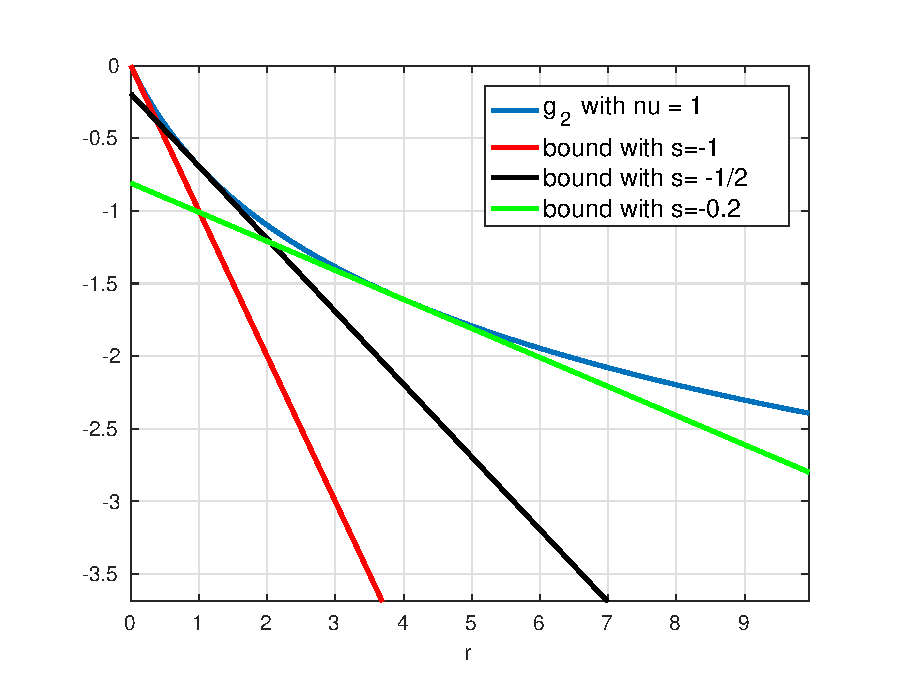
\includegraphics[width = 0.75 \textwidth]{bound}
  \caption{\label{fig:bound} Minorising linear functions for the convex $g_2(r)$. For any $r$ there is a corresponding tangent with slope $s$ and intercept $-g_2^*(s)$.}
\end{figure}

We thus obtain
\begin{align}
  - \log [1+1/\nu \exp(h(\u;\thetab))] &= g_2(r(\u;\thetab))\\
  &\ge  r(\u;\thetab)s + 1+ \nu s - \log\left[ -\frac{1}{\nu s}\right]
\end{align}
and inserting \eqref{eq:r-importance-sampling} for $r(\u;\thetab)$, we have
\begin{equation}
  - \log [1+1/\nu \exp(h(\u;\thetab))] \ge \E_{\z \sim q_u} \left[\frac{\pnn(\u,\z; \thetab)}{q_u(\z) \pnoise(\u)}\right] s  + 1+ \nu s - \log\left[ -\frac{1}{\nu s}\right].
\end{equation}
While we here use the same $q_u$ as for lower bound of the first term, it would be possible to work with a different distribution $q_u$. Moreover, we should let the value of $s$ depend on $r$, or $\u$, because for any given value of $r$, certain $s$ yield a tighter bound.

Inserting the above lower bound with $s=s(\y)$ into \eqref{eq:Jbound1} gives
\begin{align}
  J(\thetab)  \ge&  -\Ex \E_{\z \sim q(\z|\x)} \log \left[1+\nu \frac{q(\z|\x)\pnoise(\x)}{\pnn(\x,\z; \thetab)}\right] -  \nu \Ey \log \left[1+1/\nu \exp(h(\y;\thetab))\right].\\
  \ge&  -\Ex \E_{\z \sim q(\z|\x)} \log \left[1+\nu \frac{q(\z|\x)\pnoise(\x)}{\pnn(\x,\z; \thetab)}\right] \nonumber \\
  &+  \nu \Ey \E_{\z \sim q(\z|\y)} \left[\frac{\pnn(\y,\z; \thetab)}{q(\z|\y) \pnoise(\y)}\right]s(\y)  + \nu + \nu^2 s(\y) - \nu\log\left[ -\frac{1}{\nu s(\y)}\right]
\end{align}
We thus have $J(\thetab) \ge J_1(\thetab,q) \ge J_2(\thetab,q)$, with
\begin{align}
  J_2(\thetab,q) =&  -\Ex \E_{\z \sim q(\z|\x)} \log \left[1+\nu \frac{q(\z|\x)\pnoise(\x)}{\pnn(\x,\z; \thetab)}\right] \nonumber \\
  &+  \nu \Ey \E_{\z \sim q(\z|\y)} \left[\frac{\pnn(\y,\z; \thetab)}{q(\z|\y) \pnoise(\y)}\right]s(\y)  + \nu + \nu^2 s(\y) - \nu \log\left[ -\frac{1}{\nu s(\y)}\right]
  \label{eq:J2-def}
\end{align}
We can interpret $s(\y)$ as the number of noise samples $\z \mid \y$
that needed to be sampled for each of the sampled $\y$. One could use
a neural network to represent $s(\y)$ and learn its parameters by
making the bound tighter.

In this second approach, we would learn the parameters $\thetab$ by iterating:
\begin{itemize}
\item maximisation of $\J_2(\thetab,q)$ with respect to $\thetab$,
\item tightening of the bound by maximising $\J_2(\thetab,q)$ with respect to the variational distribution $q$ and with respect to the parameters of the function $s(\y)$
\end{itemize}

\emph{Remark:} The first approach seems simpler. I don't quite know whether $J_2$ has any advantages over $J_1$. Optimisation may be easier. At least it seems more amenable to stochastic gradient ascent.

\section{Sanity check}

Figures \ref{fig:density} and \ref{fig:objective} show the result of a simple simulation. The observed data were sampled from a Gaussian mixture model,
\begin{align}
  \pdata(x | z=1) &= \mathcal{N}(0,(\sigma_1^\ast)^2)\\
  \pdata(x | z=0) &= \mathcal{N}(0,(\sigma^\ast_0)^2)
  \end{align}
with  $\sigma_1^\ast = 1$ and $\sigma_0^\ast = 4$. The sample size was large to avoid random effects: $n = 100000$. The probability for $z=0$ and $z=1$ was $0.5$. Figure \ref{fig:density} visualises $\pdata(x)$.

To test the bounds, we work with the model
\begin{equation}
  \pnn(u,z; \theta) = \frac{1}{2}\mathcal{N}(0,(\sigma_1^\ast)^2)z+\frac{1}{2}\mathcal{N}(0,\theta^2)(1-z)
\end{equation}
This is a simplification because for any given value of $z \in
\{0,1\}$, the model is correctly normalised. Here,
$\mathcal{N}(0,\sigma^2)$ stands for the pdf of a Gaussian with variance $\sigma^2$.

For NCE, with sum over $z$ to obtain the mixture model
\begin{equation}
  \pnn(u,\theta) = \frac{1}{2}\mathcal{N}(0,(\sigma_1^\ast)^2)+\frac{1}{2}\mathcal{N}(0,\theta^2),
\end{equation}
which is correctly normalised (this is a simplification and has to be relaxed). The noise distribution was $\mathcal{N}(0,(\sigma^\ast_0)^2)$.

For lower bound, we work with the variational distribution $q(z| u)$ defined by
\begin{equation}
  q(z=0 | u) =\frac{1}{1+\frac{\sigma_0^\ast}{\sigma_1^\ast}\exp \left(-\frac{u^2}{2}\left(\frac{1}{(\sigma_1^\ast)^2}-\frac{1}{(\sigma_0^\ast)^2}\right)\right) }
  \label{eq:variational-example}
\end{equation}
which is the conditional distribution for $z \mid x$ derived from $\pdata(x | z)$. 

Figure \ref{fig:density} left  shows that NCE works well for the chosen noise distribution. Given the large sample size the maximiser of the NCE objective $J(\theta)$ is essentially equal to $\sigma^\ast_0$.

The right subfigure in Figure \ref{fig:density} shows
$\J_1(\theta)$. We see that $\J_1(\theta)$ is indeed a lower
bound. Its maximiser is not exactly equal to maximiser of the NCE
objective, and $\sigma^\ast_0$. This may be because the same
variational distribution was used for all $\theta$ when plotting $\J_1(\theta)$


\begin{figure}
  \centering
  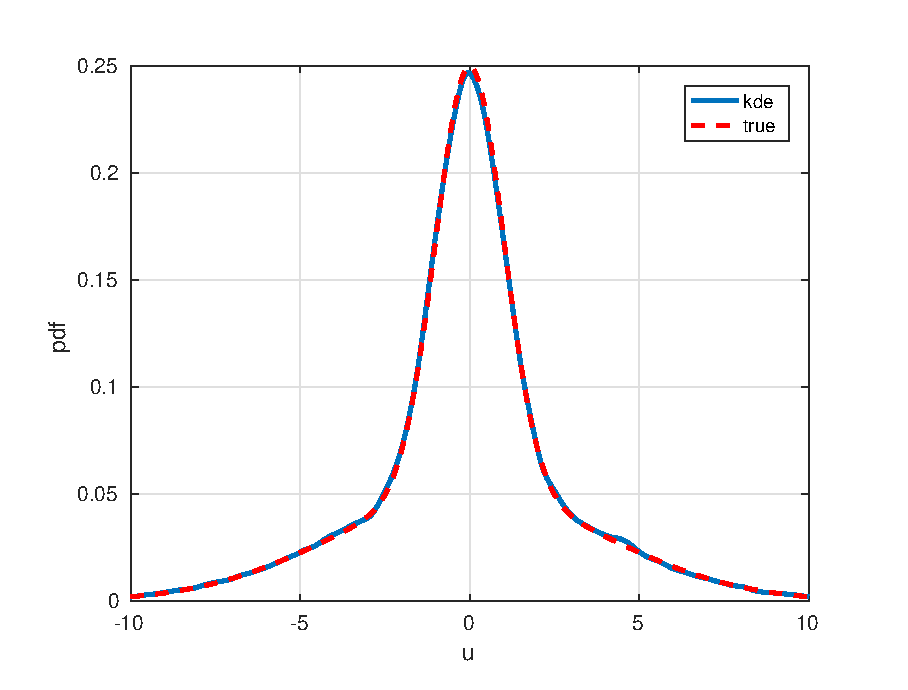
\includegraphics[width = 0.45\textwidth]{density}
  \caption{\label{fig:density} Density from which the data were sampled: It is a mixture of Gaussians; Both components of the mixture have mean 0. The first component has standard deviation 1, the second (zero-th in the code) has standard deviation $\sigma_0 = 4$. Parameter of interest is $\sigma_0$.}
\end{figure}

\begin{figure}
  \centering
  \subfloat[NCE]{ 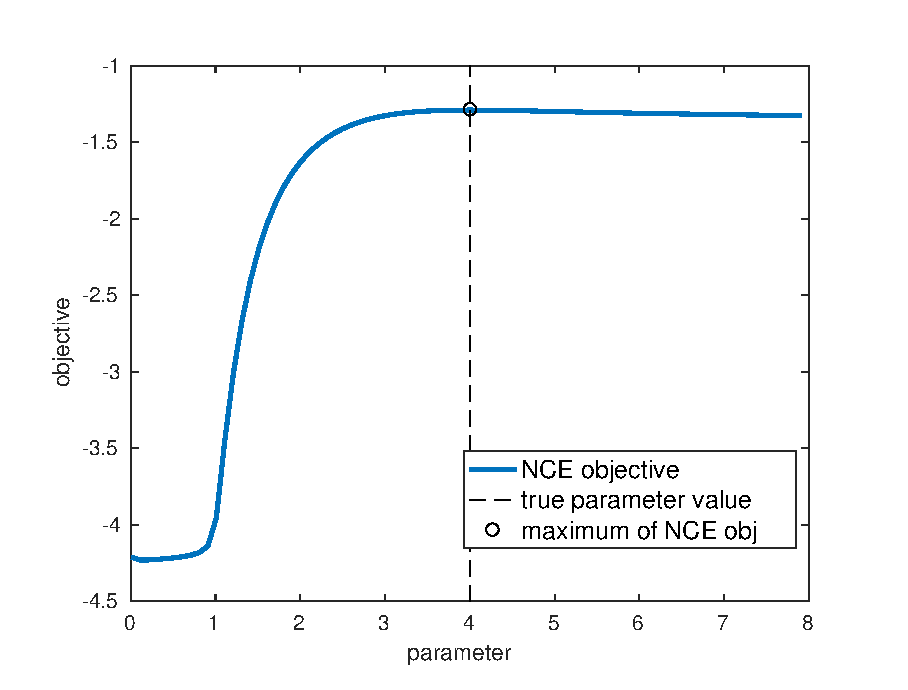
\includegraphics[width = 0.475\textwidth]{nce}}\hfill
  \subfloat[Lower bound]{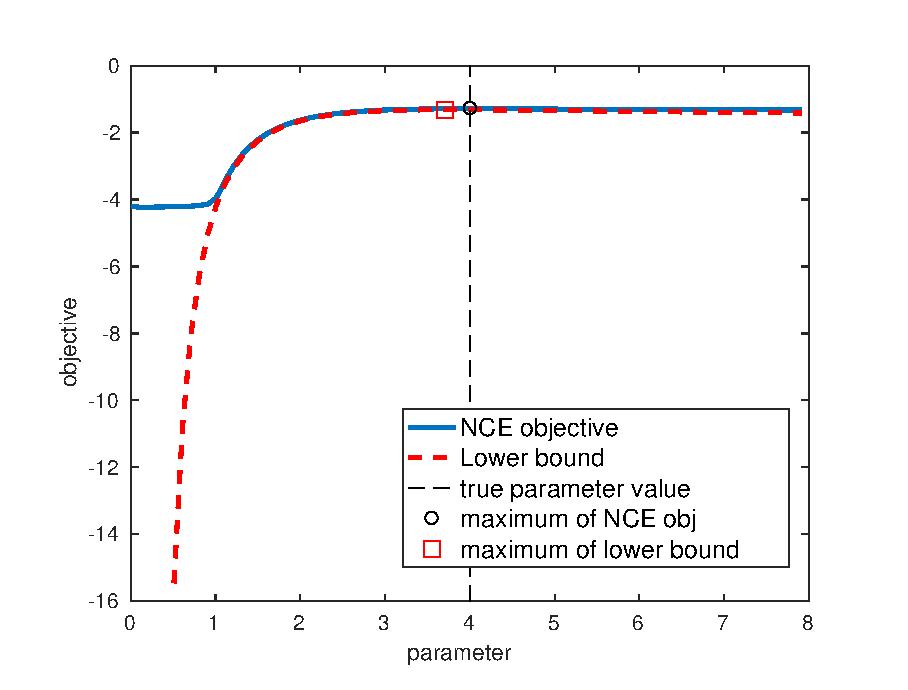
\includegraphics[width = 0.475\textwidth]{lower-bound}}
  \caption{\label{fig:objective} Left: NCE objective function after integrating out the latent variable. For simplicity, the density is assumed to be correctly normalised. This has to be relaxed; the normalisation constant has to be estimated as well. Right: Lower bound $\J_1(\thetab)$ with the same noise as for the NCE objective function. The variational distribution $q(z| u)$ is given in \eqref{eq:variational-example}.}
\end{figure}
  
\section{Next tasks}
\begin{enumerate}
\item Double-check derivations
\item Extend the code to more realistic setting: 
  \begin{enumerate}
  \item  $\phi(u,z; \theta)$ is unnormalised, 
  \item we iterate between optimisation with respect to $\theta$ and with respect to the variational distribution.
  \end{enumerate}
\item Consider smaller sample size and do some population analysis (multiple runs)
\item More challenging examples
\item Consider $\J_2(\thetab)$ (?)
\end{enumerate}

\newpage
\bibliographystyle{plainnat}
\bibliography{reference}

\end{document}  
